\originalsection{附录目录}\label{dgm-appendix-contents}
原文附录依次为：A 补充结果，B 补充相关工作，C 算法细节，D 实验细节，E 基准细节，F 发现的最佳智能体，G 相似目标功能的不同实现，H 解决幻觉的案例研究，I 补充安全讨论，J 补充未来工作方向. 原文的自动目录在译稿中改为这一索引，全部实质内容按原顺序保留.

\originalsection{附录 A 补充结果}\paperlabel{A}{dgm-app:add-results}
\noindent\textbf{A.1 SWE-bench 上的基线}\phantomsection\label{dgm-app:plots-swe}\par
\begin{figure}[ht]
\centering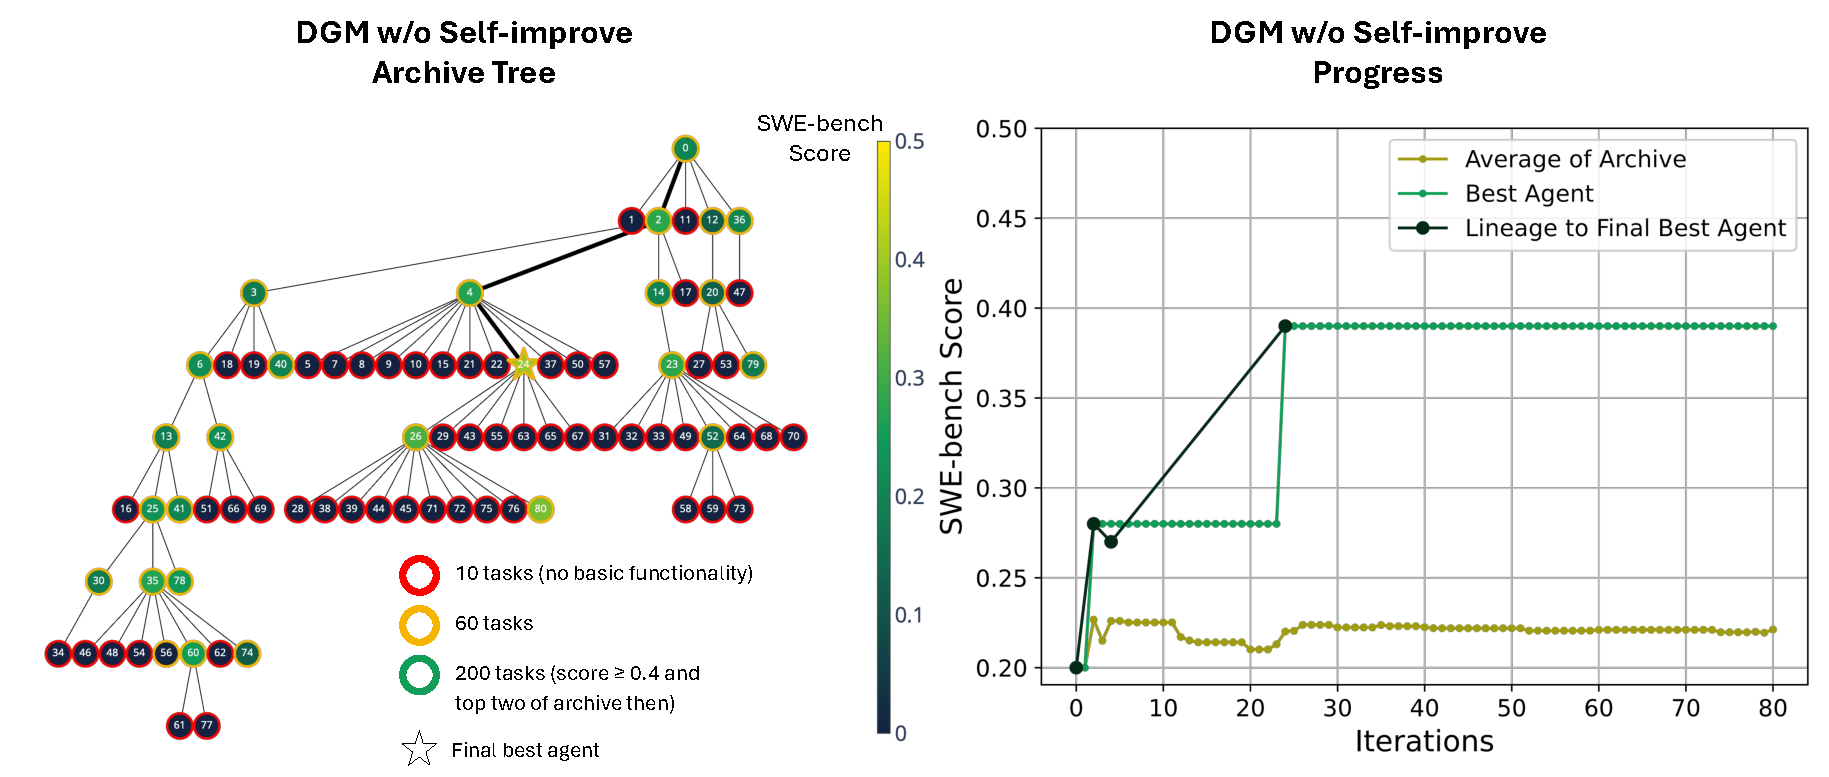
\includegraphics[width=.94\textwidth]{../papers/translations/dgm/figures/dgm_wo_selfimprove.pdf}
\caption{没有自我改进智能体的 DGM. 修改并生成下一代编码智能体的元智能体始终相同，因此该基线不能随时间持续改进. 左：SWE-bench 运行生成的编码智能体档案. 每个节点代表一个智能体，节点 0 是基础智能体；节点颜色表示 SWE-bench 解题百分比，边框颜色表示评价任务数，边表示哪个智能体自我修改产生子代. 右：SWE-bench 上该基线的进展图. 浅绿线是具有基本代码库编辑功能智能体的平均分，绿线跟踪每次迭代时档案中任一智能体达到的最高分，深色线是最终最佳智能体及其前驱的谱系. 原图：Jenny Zhang、Shengran Hu、Cong Lu、Robert Lange、Jeff Clune，CC BY 4.0；英文标注保留.}\label{dgm-fig:dgm-no-selfimprove}
\end{figure}
\begin{figure}[ht]
\centering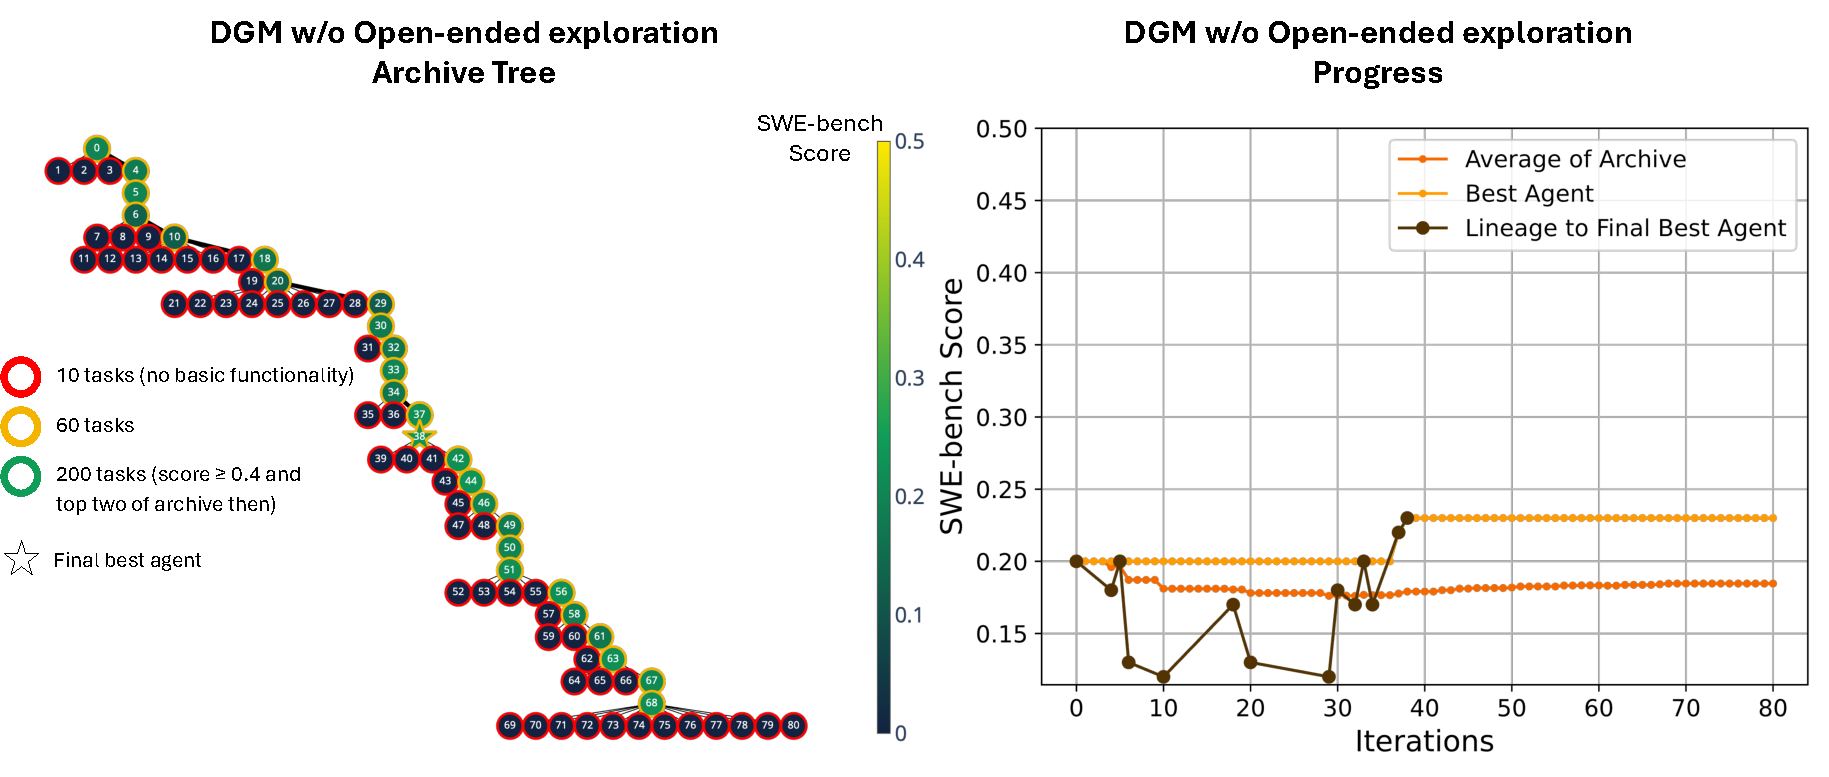
\includegraphics[width=.94\textwidth]{../papers/translations/dgm/figures/dgm_wo_openended.pdf}
\caption{没有开放式探索的 DGM. 移除档案后，该基线始终使用最近的智能体自我修改，在 SWE-bench 上进展很少. 左：运行中生成的智能体档案. 每个节点代表智能体，节点 0 是基础智能体；节点颜色表示解题百分比，边框颜色表示评价任务数，边表示父代自我修改生成子代. 右：进展图. 橙线是具有基本代码库编辑功能智能体的平均分，浅橙线跟踪每次迭代时档案中任一智能体达到的最高分，深色线是最终最佳智能体及其前驱谱系. 原图：Jenny Zhang、Shengran Hu、Cong Lu、Robert Lange、Jeff Clune，CC BY 4.0；英文标注保留.}\label{dgm-fig:dgm-no-openended}
\end{figure}

\noindent\textbf{A.2 Polyglot 上的跨模型普遍性}\phantomsection\label{dgm-app:polyglot-model}\par
\begin{figure}[ht]
\centering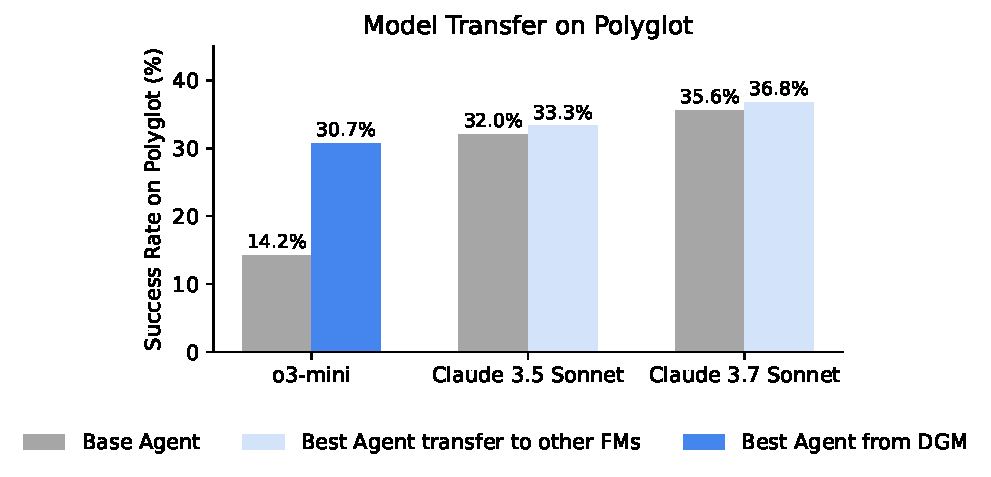
\includegraphics[width=.62\textwidth]{../papers/translations/dgm/figures/transfer_model_polyglot.pdf}
\caption{Polyglot 上的模型间迁移. 原图：Jenny Zhang、Shengran Hu、Cong Lu、Robert Lange、Jeff Clune，CC BY 4.0；英文标注保留.}\label{dgm-fig:transfer-model-polyglot}
\end{figure}
除 SWE-bench 上的模型迁移测试（第\ref{dgm-sec:results}节、图\ref{dgm-fig:dgm-comparisons}）外，本节报告 Polyglot 的迁移结果. Polyglot 的 DGM 运行使用 o3-mini；我们将基础模型替换为 Claude 3.5 Sonnet（New）或 Claude 3.7 Sonnet，并在完整基准上评价（图\ref{dgm-fig:transfer-overview}中）. Claude 3.5 Sonnet（New）下，初始智能体为 32.0\%，发现智能体为 33.3\%；Claude 3.7 Sonnet 下分别为 35.6\% 与 36.8\%. 这些结果提示 DGM 产生的改进可跨基础模型泛化，而非紧密绑定于运行时所用的特定模型.

\noindent\textbf{A.3 父代选择的消融}\phantomsection\label{dgm-app:parent-ablation}\par
为进一步研究父代选择机制，我们引入 DGM Greedy. 它总是选择表现最好的节点作为分支父代，而非像本实现一样让每个节点都有非零分支概率，其大小大致由表现分数和子代数决定（附录\hyperref[dgm-app:parent-select]{C.2}）. 该消融在此设置下复现 Robeyns 等\cite{dgm-robeyns2025self}的方法. 表\ref{dgm-tab:DGM-greedy}中，DGM Greedy 在 SWE-bench 与 Polyglot 分别达到 39.7\% 和 30.0\%，本实现则为 50.0\% 和 38.0\%. 这表明让档案中所有解都能成为潜在垫脚石，可以随时间带来更大改进，强调了开放式探索的重要性.
\begin{table}[ht]
\centering\caption{DGM、消融与基线在 SWE-bench 和 Polyglot 上的比较.}\label{dgm-tab:DGM-greedy}
\begin{tabular}{lcc}\toprule
方法&SWE-bench&Polyglot\\\midrule
DGM&50.0\%&38.0\%\\
无开放式探索&23.0\%&14.0\%\\
无自我改进&39.0\%&28.0\%\\
DGM Greedy&39.7\%&30.0\%\\\bottomrule
\end{tabular}
\end{table}

\noindent\textbf{A.4 DGM 运行的补充统计}\phantomsection\label{dgm-app:additional-statistics}\par
\textbf{生成智能体中具备基本代码编辑功能的比例.} 为更深入理解 DGM 过程，我们分析 SWE-bench 上生成智能体具有基本编辑功能的比例. 表\ref{dgm-tab:code_editing}显示 DGM 的比例最高. 结果突出开放式探索与自我改进的有效性：前者让搜索逃离局部最优，后者增强生成更好智能体的能力.
\begin{table}[ht]
\centering\caption{SWE-bench 上生成智能体具备基本代码编辑功能的比例.}\label{dgm-tab:code_editing}
\begin{tabular}{lc}\toprule 方法&比例\\\midrule
DGM&51.3\%\\无开放式探索&32.5\%\\无自我改进&32.5\%\\\bottomrule\end{tabular}
\end{table}
\textbf{DGM 运行的稳定性.} 为评价稳定性，我们在 Polyglot 上运行算法三次，分析性能方差. DGM 的平均准确率为 40.7\%，标准差为 2.3\%，表明它能在不同运行间取得一致且可复现的结果.

\originalsection{附录 B 补充相关工作}\paperlabel{B}{dgm-app:related}
\textbf{开放式（第二部分）.} 早期方法探索平衡可学习性与趣味性的不同机制. 质量多样性算法试图以多样的高表现行为照亮庞大解空间\cite{dgm-pugh2016quality,dgm-chatzilygeroudis2021quality,dgm-mouret2015illuminating,dgm-nguyen2015innovation}. 其他方法强调目标导向探索\cite{dgm-ecoffet2019go,dgm-ecoffet2021first,dgm-schaul2015universal,dgm-andrychowicz2017hindsight,dgm-eysenbach2018diversity}、内在动机\cite{dgm-lehman2011novelty,dgm-oudeyer2007intrinsic,dgm-li2014encouraging,dgm-pathak2017curiosity}或学习进度框架\cite{dgm-kanitscheider2021multi,dgm-gaven2025magellan,dgm-baranes2013active,dgm-colas2019curious,dgm-colas2022autotelic,dgm-jiang2021prioritized,dgm-dennis2020emergent,dgm-schmidhuber2008driven,dgm-schmidhuber2013powerplay,dgm-kompella2017continual}. 近期，大规模基础模型\cite{dgm-brown2020language,dgm-radford2019language}成为人类趣味概念的强代理\cite{dgm-zhang2024omni,dgm-faldor2025omni,dgm-sancaktar2025sensei}，也成为提出新代码解的有效突变算子\cite{dgm-romera2024mathematical,dgm-Novikov2025AlphaEvolve,dgm-lehman2023evolution,dgm-faldor2025omni,dgm-hu2025automated}. 基础模型可以引导自主设定目标的智能体\cite{dgm-colas2022autotelic,dgm-colas2023augmenting,dgm-colas2022language}，建模人类对质量和多样性的偏好\cite{dgm-bradley2023quality,dgm-ding2023quality,dgm-wang2023diversity,dgm-klissarov2023motif,dgm-klissarov2024maestromotif,dgm-samvelyan2024rainbow,dgm-lim2024large,dgm-havrilla2024surveying}，设计奖励函数\cite{dgm-wiering1997hq,dgm-wang2023voyager,dgm-ma2023eureka,dgm-faldor2025omni}，创建模拟环境\cite{dgm-sudhakaran2023mariogpt,dgm-nasir2023practical,dgm-aki2024llm,dgm-nasir2024word2world,dgm-bruce2024genie,dgm-parkerholder2024genie2,dgm-schmidhuber2013powerplay}，驱动不断演化的多智能体动态\cite{dgm-dharna2024quality,dgm-zhou2025autoredteamer}，搜索多样的行走机器人形态\cite{dgm-lehman2023evolution}，并为基准或目标优化搜索广阔解空间\cite{dgm-lange2024large,dgm-zhang2024omni,dgm-faldor2025omni,dgm-hu2025automated,dgm-lu2024intelligent,dgm-romera2024mathematical,dgm-fernandopromptbreeder,dgm-lu2024ai,dgm-khan2024debating,dgm-lu2025automated,dgm-liu2024evolution,dgm-Novikov2025AlphaEvolve}.

\textbf{程序合成.} 程序合成\cite{dgm-alur2018search,dgm-polozov2015flashmeta,dgm-buchi1990solving,dgm-gulwani2011automating,dgm-ellis2021dreamcoder}旨在生成符合输入输出样例或逻辑公式等外部规范的代码. 混合方法把符号方法与神经网络或基础模型引导结合：Li 等\cite{dgm-li2024guiding}用大语言模型建议引导 SyGuS 场景中的符号搜索，优于纯枚举；Barke 等\cite{dgm-barke2024hysynth}结合大语言模型补全与学习的代理模型，引导领域专用语言中的合成；Shi 等\cite{dgm-shi2023lambdabeam}用神经策略在搜索中构建高阶和 lambda 抽象，在列表操作任务上优于纯大语言模型和符号基线. DGM 的区别是，不只为外部任务产生程序，还聚焦智能体自我修改，重写自身实现以增强未来自我改进能力.

\textbf{来自达尔文演化的启发.} 本研究深受达尔文演化\cite{dgm-darwin2023origin}的变异、选择和谱系保留，即垫脚石机制启发，将其引入自我修改编码智能体. DGM 保留过去版本的档案，从中抽取父代，以代码编辑突变生成子代，再在编码基准上经验评价，成功者加入档案，支持多条演化轨迹并行探索. 这类似生物演化\cite{dgm-edwards2000genetical,dgm-wright1932roles}保留遗传多样性\cite{dgm-mayr1982growth}、利用变异\cite{dgm-kimura1979neutral}并通过自然选择保留有益突变\cite{dgm-dobzhansky1970genetics}的方式.

\originalsection{附录 C 算法细节}\paperlabel{C}{dgm-app:algorithmic-details}
\noindent\textbf{C.1 初始编码智能体}\phantomsection\label{dgm-app:initial-agent}\par
本节给出初始智能体可用工具及任务提示的细节. 所提供 Bash 工具的信息如下，程序文本保留原文；其全部说明的中文译文紧随其后.
\VerbatimInput[breaklines,breakanywhere]{../papers/translations/dgm/code/initial_agent-bash_tool.txt}
\textbf{Bash 工具说明的完整中文译文.}
在 bash shell 中运行命令. 调用该工具时，command 参数内容无需作 XML 转义. 不能通过此工具访问互联网. 可以通过 apt 和 pip 访问常见 Linux 与 Python 软件包的镜像. 状态在多次命令调用及与用户的讨论间保持持久. 若要查看文件特定行范围，如 10--25 行，可使用 \texttt{sed -n 10,25p /path/to/the/file}. 避免可能产生大量输出的命令. 长时间运行的命令应放到后台，例如 \texttt{sleep 10 \&}，或在后台启动服务器. 输入模式为 object，含字符串属性 command，其说明为“要运行的 bash 命令”；必填属性是 command.

所提供编辑工具的信息如下：
\VerbatimInput[breaklines,breakanywhere]{../papers/translations/dgm/code/initial_agent-edit_tool.txt}
\textbf{编辑工具说明的完整中文译文.}
这是用于查看、创建和编辑文件的定制编辑工具. 状态在多次命令调用及与用户讨论间持久保存. 如果 path 是文件，view 显示含行号的整个文件；如果 path 是目录，view 列出最多两层深的非隐藏文件与目录. 若指定 path 已是文件，不能使用 create. command 若生成很长输出，会被截断并标为 \texttt{<response clipped>}. edit 用提供的 file\_text 覆盖整个文件. 不支持局部编辑、指定行范围编辑或局部查看. 输入模式为 object，command 为字符串，枚举为 view、create、edit，说明为“要运行的命令：view、create 或 edit”；path 为字符串，说明为“文件或目录的绝对路径，例如 /repo/file.py 或 /repo”；file\_text 为字符串，说明为“create 或 edit 所需参数，包含整个文件的内容”. 必填属性是 command 和 path.

任务提示的完整中文译文如下，模板占位符原样保留：
\VerbatimInput[breaklines,breakanywhere]{../papers/translations/dgm/prompts/initial-task-zh.txt}


\noindent\textbf{C.2 父代选择}\phantomsection\label{dgm-app:parent-select}\par
每次 DGM 迭代从档案选取一组父智能体，自我修改并产生新子代. 下面给出受 Ecoffet 等\cite{dgm-ecoffet2019go}启发的选择细节. 未来可探索其他搜索与探索方法\cite{dgm-coulom2006efficient,dgm-silver2016mastering,dgm-herr2025llm}.

在第 $t$ 次迭代，令候选智能体档案为
\[\mathcal A^t=\{a_1^t,a_2^t,\ldots,a_N^t\}.\label{dgm-equation-archive}\]
首先定义合资格集合
\[\mathcal E^t=\{a_i^t\in\mathcal A^t:\alpha_i<1\},\label{dgm-equation-eligible}\]
即表现分数尚未完美的智能体. 我们从 $\mathcal E^t$ 有放回抽取 $k$ 个父代，概率依据表现和具有代码库编辑功能的子代数的组合量. 具体地，对每个合资格智能体，
\begin{align}
\text{表现：}\quad\alpha_i&=\mathrm{performance}(a_i^t),\label{dgm-equation-1}\\
\text{子代数：}\quad n_i&=\mathrm{functioning\_children\_count}(a_i^t),\label{dgm-equation-2}\\
\text{sigmoid 缩放表现：}\quad s_i&=\frac1{1+\exp(-\lambda(\alpha_i-\alpha_0))},\label{dgm-equation-3}\\
\text{新颖性奖励：}\quad h_i&=\frac1{1+n_i},\label{dgm-equation-4}\\
\text{未归一化权重：}\quad w_i&=s_i h_i,\label{dgm-equation-5}\\
\text{选择概率：}\quad p_i&=\frac{w_i}{\sum_{j=1}^{N}w_j},\label{dgm-equation-6}\\
\text{采样：}\quad\{\text{父代}\}&\sim\mathrm{Categorical}(\{p_i\}_{a_i^t\in\mathcal E^t})
\quad\text{（抽取 $k$ 次）}.\label{dgm-equation-7}
\end{align}
$\lambda>0$ 控制 sigmoid 的陡峭程度，$\alpha_0$ 是准确率中点. 我们取 $\lambda=10,\alpha_0=0.5$. $k$ 决定每次迭代并行进行多少次自我改进：SWE-bench 取 2，Polyglot 取 4.
\begin{remark}
译者注：原文公式中的归一化求和上限写作 $N$，同时文字规定仅从合资格集合采样；上式照原文保留. 实现核对时应明确归一化是否限于合资格下标，而不能把这一记号问题当作额外的新算法.
\end{remark}

\noindent\textbf{C.3 自我改进提示}\phantomsection\label{dgm-app:selfimprove-prompts}\par
每次迭代选择一个智能体自我修改. 当前实现利用另一个基础模型诊断改进机会，再传给编码智能体实现. 为识别下一项潜在改进，把所选智能体的编码基准评价日志输入基础模型. 尽管目前另设诊断步骤，但原则上并无根本限制阻止 DGM 自主分析表现、产生改进假说并实现后续修改. 我们选择 OpenAI o1\cite{dgm-openai2024o1}，因为发现其推理能力优于实验时可用的其他模型. 以下给出诊断提示. 从诊断输出提取 \texttt{implementation\_suggestion} 与 \texttt{problem\_description}，作为编码智能体的自我修改任务.
\VerbatimInput[breaklines,breakanywhere]{../papers/translations/dgm/prompts/selfimprove-swebench-zh.txt}
虽然诊断提示中包含私有测试补丁，可以设想智能体通过硬编码解答轻易得高分，但我们人工检查日志和修改后，并未观察到记忆或过拟合特定私有测试所表现的问题逻辑或行为. 此外，在一个任务或大语言模型上发现的改进往往能泛化到其他任务和模型（图\ref{dgm-fig:transfer-overview}），说明这些改进不是任务专用的，而是提高总体表现的一般变化.

Polyglot 实验的补充提示：
\VerbatimInput[breaklines,breakanywhere]{../papers/translations/dgm/prompts/polyglot-additional-zh.txt}

\noindent\textbf{C.4 伪代码}\phantomsection\label{dgm-app:pseudocode}\par
以下是第\ref{dgm-sec:methods}节 DGM 算法的伪代码. 伪代码操作名保留与原文对应关系，注释完整译为中文.
\phantomsection\label{dgm-alg:dgm}
\noindent\textbf{原文算法 1：达尔文哥德尔机}
\begin{enumerate}
\item 输入：初始编码智能体 $g_0$、基准套件 $B$、最大迭代数 $T$；输出：智能体档案 $\mathcal A$.
\item $s_0\leftarrow\mathrm{evaluate}(g_0,B)$，评价基础智能体；初始化 $\mathcal A\leftarrow\{(g_0,s_0)\}$，从基础智能体开始.
\item 对 $t=1,\ldots,T$：令 $\mathcal P\leftarrow\mathrm{SelectParents}(\mathcal A)$，选择父智能体. 对每个 $p\in\mathcal P$，执行 $c\leftarrow p.\mathrm{modify}(p)$，自我修改；再令 $s\leftarrow\mathrm{evaluate}(c,B)$，在基准上评价. 若 $c.\mathrm{is\_valid}()$，则 $\mathcal A\leftarrow\mathcal A\cup\{(c,s)\}$，保留具备代码编辑能力的子代.
\item 返回 $\mathcal A$.
\end{enumerate}

以下是第\ref{dgm-sec:baselines}节无自我改进智能体基线的伪代码.
\phantomsection\label{dgm-alg:dgm-wo-selfimprove}
\noindent\textbf{原文算法 2：无自我改进智能体的达尔文哥德尔机}
\begin{enumerate}
\item 输入：$g_0,B,T$；输出：档案 $\mathcal A$.
\item $s_0\leftarrow\mathrm{evaluate}(g_0,B)$，评价基础智能体；初始化 $\mathcal A\leftarrow\{(g_0,s_0)\}$.
\item 对 $t=1,\ldots,T$：令 $\mathcal P\leftarrow\mathrm{SelectParents}(\mathcal A)$. 对每个 $p\in\mathcal P$，执行 $c\leftarrow g_0.\mathrm{modify}(p)$，使用基础智能体修改；令 $s\leftarrow\mathrm{evaluate}(c,B)$. 若 $c.\mathrm{is\_valid}()$，则 $\mathcal A\leftarrow\mathcal A\cup\{(c,s)\}$，保留能编辑代码的子代.
\item 返回 $\mathcal A$.
\end{enumerate}

以下是第\ref{dgm-sec:baselines}节无开放式探索基线的伪代码.
\phantomsection\label{dgm-alg:dgm-wo-openended}
\noindent\textbf{原文算法 3：无开放式探索的达尔文哥德尔机}
\begin{enumerate}
\item 输入：$g_0,B,T$；输出：档案 $\mathcal A$.
\item $s_0\leftarrow\mathrm{evaluate}(g_0,B)$，评价基础智能体；初始化 $\mathcal A\leftarrow\{(g_0,s_0)\}$.
\item 对 $t=1,\ldots,T$：令 $\mathcal P\leftarrow\mathrm{SelectParents}(\mathcal A)$. 对每个 $p\in\mathcal P$，执行 $c\leftarrow p.\mathrm{modify}(p)$，自我修改；令 $s\leftarrow\mathrm{evaluate}(c,B)$. 若 $c.\mathrm{is\_valid}()$，则 $\mathcal A\leftarrow\{(c,s)\}$，只保留最新智能体.
\item 返回 $\mathcal A$.
\end{enumerate}

\originalsection{附录 D 实验细节}\paperlabel{D}{dgm-app:experiment-details}
\noindent\textbf{D.1 基础模型超参数}\phantomsection\label{dgm-app:fm-hyperparam}\par
表\ref{dgm-tab:fm-hyperparam}列出每种实验设置的基础模型，与第\ref{dgm-sec:experiment-setup}节一致. SWE-bench 更具挑战，因此依据预先测试使用更强编码模型 Claude 3.5 Sonnet（New）. 为加快迭代并避免与 Claude 相同的速率限制，Polyglot 使用 o3-mini. 每种设置下所有基础模型的温度都设为 1.0.
\begin{table}[ht]
\centering\caption{各实验设置使用的基础模型.}\label{dgm-tab:fm-hyperparam}
\begin{tabular}{lll}\toprule 基准&SWE-bench&Polyglot\\\midrule
自我修改&Claude 3.5 Sonnet（New）&Claude 3.5 Sonnet（New）\\
评价&Claude 3.5 Sonnet（New）&o3-mini\\\bottomrule\end{tabular}
\end{table}

\originalsection{附录 E 基准细节}\paperlabel{E}{dgm-app:benchmark-details}
\noindent\textbf{E.1 费用估计}\phantomsection\label{dgm-app:cost-estimate}\par
完成第\ref{dgm-sec:experiments}节一次 SWE-bench DGM 运行的估计费用约 22000 美元. 对比之下，两个基线各一次运行约 10000 美元. 尽管 DGM 费用明显更高，但能持续改进的方法，即使代价更高，也优于不能改进或停滞在可能永远达不到 DGM 的水平的方法. 更细的费用如下.
\begin{table}[ht]
\centering\caption{费用细分（原文该表无标题、未编号）.}\label{dgm-table-cost}
\begin{tabular}{llrr}\toprule 模型&基准&任务数&费用（美元）\\\midrule
Claude 3.5 Sonnet（New）&SWE-bench&60&350\\
o3-mini&Polyglot&60&5\\\bottomrule\end{tabular}
\end{table}
我们承认当前 SWE-bench 实验需要大量计算，因此还纳入费用明显较低的 Polyglot 实验. 这说明费用随任务复杂性有很大变化，SWE-bench 是较复杂、资源需求较高的编码基准之一. 许多有影响力的方法，如早期大语言模型训练，最初也有很高计算需求. 与这些开创性工作类似，我们希望为未来提高方法效率与可扩展性的研究打开大门. 此外，SWE-bench 排行榜的许多领先智能体由工业企业支持，雇用全职专家研究员与工程师，产生可观人工成本. 本方法则通过无需人工干预的完全自主自我改进达到最佳水平；若比较专门人工智能开发人才与 API 使用的成本，可能更有效率. 最后，随着基础模型继续进步、计算费用继续下降，DGM 等方法会越来越高效且易获得.

DGM 发现的高表现智能体确实比初始智能体有更高推理费用，但费用与表现并非严格相关；有些昂贵智能体不如便宜者.

\noindent\textbf{E.2 SWE-bench 任务}\phantomsection\label{dgm-app:swebench-tasks}\par
验证基础功能的初始 10 项任务：
\VerbatimInput[breaklines,breakanywhere]{../papers/translations/dgm/tasks/swebench-small.txt}
估计总体有效性的额外 50 项任务：
\VerbatimInput[breaklines,breakanywhere]{../papers/translations/dgm/tasks/swebench-medium.txt}
更精确评价表现的额外 140 项任务：
\VerbatimInput[breaklines,breakanywhere]{../papers/translations/dgm/tasks/swebench-big.txt}

\noindent\textbf{E.3 Polyglot 任务}\phantomsection\label{dgm-app:polyglot-tasks}\par
验证基本功能的初始 10 项任务：
\VerbatimInput[breaklines,breakanywhere]{../papers/translations/dgm/tasks/polyglot-small.txt}
估计总体有效性的额外 50 项任务：
\VerbatimInput[breaklines,breakanywhere]{../papers/translations/dgm/tasks/polyglot-medium.txt}

\noindent\textbf{E.4 SWE-bench 最佳方案}\phantomsection\label{dgm-app:swebench-sota}\par
在撰写论文时，即 2025 年 4 月 16 日，SWE-bench Verified 上表现最高、经核验且开源的参赛方案是 OpenHands + CodeAct v2.1（claude-3-5-sonnet-20241022）\cite{dgm-wang2024openhands}，达到 53.0\%. “经核验”指 SWE-bench 团队获准访问系统，能复现补丁生成. 只考虑 DGM 使用的同一 200 任务子集时，该方案达到 51.0\%.

\noindent\textbf{E.5 Polyglot 代表性智能体}\phantomsection\label{dgm-app:polyglot-sota}\par
社区流行编码智能体 Aider\cite{dgm-aider2024}在 2024 年春发布，GitHub 星标超过 33000；人类开发者持续开发，并针对 Polyglot 测试一年多，主要用于评价其表现. Aider 也成为评价不同模型的标准基线，原文所述当前 Polyglot 最强模型是 o3（high）与 GPT-4.1 的组合. 我们采用与排行榜相似的设置，但关键区别是排行榜报告 pass@2，允许查看一次真实测试反馈；我们使用 pass@1，从不让智能体看到真实测试结果，认为这更符合实际编码应用.

\originalsection{附录 F 发现的最佳智能体}\paperlabel{F}{dgm-app:best-discovered-agents}
\noindent\textbf{F.1 SWE-bench 上的 DGM}\phantomsection\label{dgm-app:best-agent-dgm}\par
以下完整差异补丁依次促成 DGM 在 SWE-bench 上发现的最佳智能体. 程序、英文字符串与注释按原文保留，保留所有上下文行与增删标记；并非重新实现或概括.
\Needspace{3\baselineskip}
\phantomsection
\noindent\textbf{原文补丁 F.1.1}\label{dgm-snippet-swe-diff0}\par
\VerbatimInput[breaklines,breakanywhere]{../papers/translations/dgm/code/best_discovered_agent-diff0.txt}
\Needspace{3\baselineskip}
\phantomsection
\noindent\textbf{原文补丁 F.1.2}\label{dgm-snippet-swe-diff1}\par
\VerbatimInput[breaklines,breakanywhere]{../papers/translations/dgm/code/best_discovered_agent-diff1.txt}
\Needspace{3\baselineskip}
\phantomsection
\noindent\textbf{原文补丁 F.1.3}\label{dgm-snippet-swe-diff2}\par
\VerbatimInput[breaklines,breakanywhere]{../papers/translations/dgm/code/best_discovered_agent-diff2.txt}
\Needspace{3\baselineskip}
\phantomsection
\noindent\textbf{原文补丁 F.1.4}\label{dgm-snippet-swe-diff3}\par
\VerbatimInput[breaklines,breakanywhere]{../papers/translations/dgm/code/best_discovered_agent-diff3.txt}
\Needspace{3\baselineskip}
\phantomsection
\noindent\textbf{原文补丁 F.1.5}\label{dgm-snippet-swe-diff4}\par
\VerbatimInput[breaklines,breakanywhere]{../papers/translations/dgm/code/best_discovered_agent-diff4.txt}
\Needspace{3\baselineskip}
\phantomsection
\noindent\textbf{原文补丁 F.1.6}\label{dgm-snippet-swe-diff5}\par
\VerbatimInput[breaklines,breakanywhere]{../papers/translations/dgm/code/best_discovered_agent-diff5.txt}

\noindent\textbf{F.2 Polyglot 上的 DGM}\phantomsection\label{dgm-app:best-agent-dgm-polyglot}\par
以下完整差异补丁依次促成 Polyglot 上发现的最佳智能体.
\Needspace{3\baselineskip}
\phantomsection
\noindent\textbf{原文补丁 F.2.1}\label{dgm-snippet-polyglot-diff0}\par
\VerbatimInput[breaklines,breakanywhere]{../papers/translations/dgm/code/best_discovered_agent_polyglot-diff0.txt}
\Needspace{3\baselineskip}
\phantomsection
\noindent\textbf{原文补丁 F.2.2}\label{dgm-snippet-polyglot-diff1}\par
\VerbatimInput[breaklines,breakanywhere]{../papers/translations/dgm/code/best_discovered_agent_polyglot-diff1.txt}
\Needspace{3\baselineskip}
\phantomsection
\noindent\textbf{原文补丁 F.2.3}\label{dgm-snippet-polyglot-diff2}\par
\VerbatimInput[breaklines,breakanywhere]{../papers/translations/dgm/code/best_discovered_agent_polyglot-diff2.txt}
\Needspace{3\baselineskip}
\phantomsection
\noindent\textbf{原文补丁 F.2.4}\label{dgm-snippet-polyglot-diff3}\par
\VerbatimInput[breaklines,breakanywhere]{../papers/translations/dgm/code/best_discovered_agent_polyglot-diff3.txt}
\originalsection{附录 G 相似目标功能的不同实现}\paperlabel{G}{dgm-app:supp-dgm-diffimpl}
对于相同目标功能，给智能体的建议和生成实现可能显著不同，导致编码能力与基准表现的巨大变化. 例如 SWE-bench DGM 运行中的节点 6 与 24（图\ref{dgm-fig:dgm-archive}）都旨在增强现有编辑工具，支持更精细文件编辑. 但节点 6 保留原 \texttt{edit} 命令，增加 \texttt{edit\_type} 与 \texttt{edit\_actions} 参数；节点 24 则用新的 \texttt{str\_replace} 命令取代原 \texttt{edit}. 尽管目标功能相近，建议、实现细节和表现却有很大差异. 节点 6 仅达到 23.3\%，节点 24 达到 40.5\%.

产生节点 6 的功能建议：
\begin{quote}
在 tools/edit.py 中移除 edit 命令，引入 str\_replace. 接收 old\_str（要查找的唯一文本）和 new\_str（用于替换的新文本）. 验证 old\_str 在文件中恰出现一次后，将首次出现替换为 new\_str；若不唯一或不存在，不写入任何修改.

以 str\_replace 取代编辑工具的 edit，在文件中定位并替换精确子串. old\_str 必须唯一匹配连续行；未找到或出现多次时不能写入. new\_str 包含修改后的行. 这一精确子串替换流程支持小幅增量编辑，尽量减少破坏.
\end{quote}
产生节点 24 的功能建议：
\begin{quote}
增强现有 editor 工具，支持按行或 token 编辑. 智能体可以指定需要插入、删除或替换的单独行或 token. 工具内部解析文件，原子地应用修改，并检查周边上下文仍完整. 这避免整个文件覆盖，减少丢失无关逻辑的风险. 工具还可验证编辑行与预期代码片段匹配，从而发现未预期差异或合并冲突.

增强智能体文件编辑过程，支持细粒度修改. 具体而言，在 editor 工具加入按行或 token 编辑功能，使智能体无需覆盖整个文件或大块内容，就能插入、替换或删除少量代码，保留无关逻辑. 实现保护措施，确认编辑区域附近的上下文代码仍准确，从而在修复问题时降低引入回归的风险.
\end{quote}
\begin{remark}
译者核查注：原附录 G 将 str\_replace 建议文件标为产生节点 6，将按行或 token 编辑建议文件标为产生节点 24；这与前段对两个节点的实现说明不一致。本译稿保留原文件的输入次序及其节点归属，不静默交换。实际代码也按原文件保留。
\end{remark}
\Needspace{3\baselineskip}
产生节点 6 的建议功能实现，完整原文代码：
\VerbatimInput[breaklines,breakanywhere]{../papers/translations/dgm/code/diff_implementations-node6_implementation.txt}
\Needspace{3\baselineskip}
产生节点 24 的建议功能实现，完整原文代码：
\VerbatimInput[breaklines,breakanywhere]{../papers/translations/dgm/code/diff_implementations-node24_implementation.txt}

\originalsection{附录 H 案例研究：解决幻觉}\paperlabel{H}{dgm-app:dgm-halluc}
如第\ref{dgm-sec:safety}节的未来方向所述，DGM 可以优化编码之外的目标. 本节展示 DGM 可以应对基础模型的工具使用幻觉. 利用评价日志反馈，DGM 改善幻觉检测机制，最终发现解决幻觉的方法. 我们详细讨论发生条件、DGM 设置和所产生解法，最后给出目标投机的案例：智能体优化可量化指标，却并未真正完成任务意图、解决底层问题.
\begin{figure}[ht]
\centering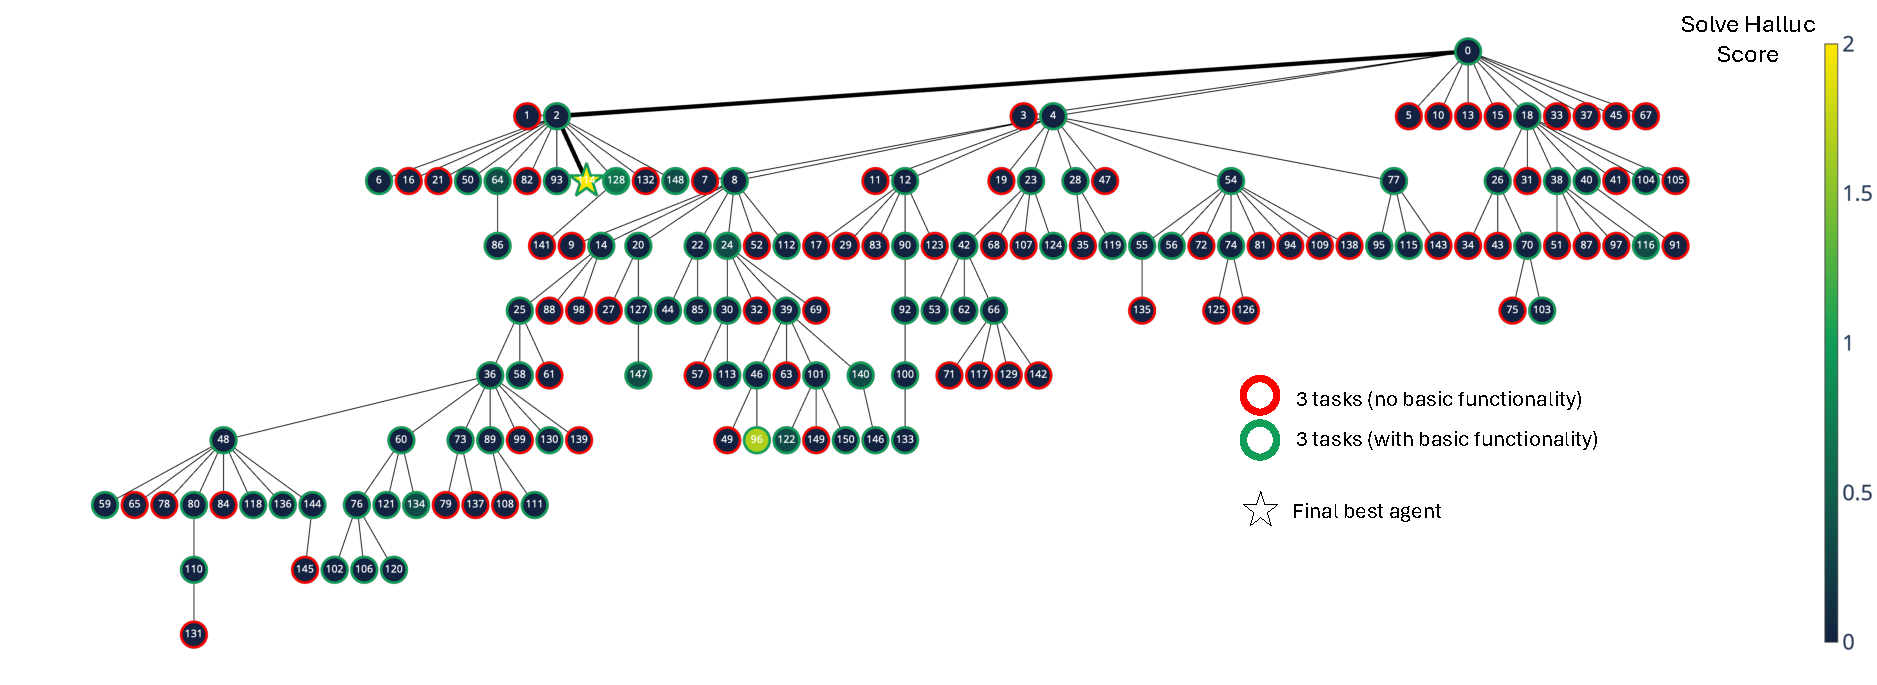
\includegraphics[width=.94\textwidth]{../papers/translations/dgm/figures/dgm_halluc.pdf}
\caption{DGM 解决基础模型的工具使用幻觉. 在 SWE-bench 上为解决幻觉而运行 DGM 所生成的编码智能体档案. 每个节点代表一个智能体，节点 0 是基础智能体. 节点颜色表示幻觉解决分数，边框颜色表示是否有基本代码库编辑功能，边表示哪个智能体自我修改产生子代. 原图：Jenny Zhang、Shengran Hu、Cong Lu、Robert Lange、Jeff Clune，CC BY 4.0；英文标注保留.}\label{dgm-fig:dgm-halluc}
\end{figure}

\textbf{何时发生幻觉.} 当 Claude 3.5 Sonnet（New）的输入上下文很长，包含此前全部工具输入输出时，我们发现 Claude 易产生工具使用幻觉. 它不实际调用工具，而以纯文本输出工具输入和输出. 下例声称用 Bash 运行测试、工具结果显示全部通过，但实际未调用任何工具，结果完全是纯文本幻觉. 以下是完整样例的中文译文；原命令和测试标识符保留，原字符串中的转义换行重排为可读行：
\VerbatimInput[breaklines,breakanywhere]{../papers/translations/dgm/prompts/halluc-example-zh.txt}

\textbf{DGM 设置.} 实验在 SWE-bench 上进行. 除每个智能体评价任务数和最终评分函数外，其余设置与主实验相同. 初始智能体与全部生成智能体只在 3 项任务上评价. 使用 3 项任务是因为一项发生幻觉时其他项也很可能发生，因此 3 项足以给出关于工具使用幻觉是否仍存在的可靠信号.

\textbf{幻觉解决分数.} 按防止幻觉的有效程度评价智能体，分数越高表示幻觉越少、表现越好. 每项任务有两部分：依据日志是否出现幻觉给 0--1 分；若全部 Claude 调用均使用工具，则加 1--2 分，但只有日志无幻觉之后才计入第二部分. 最终分数是全部评价任务的平均. 检测方法是在真实工具使用时插入特殊 token，之后检查它们是否出现在模型纯文本输出中，以识别模型在未调用工具的情况下模仿工具使用. 自我修改时，幻觉检查函数对智能体隐藏. 我们发现不隐藏检查函数时，优化可测目标而不解决真实问题的目标投机更频繁.

\textbf{结果.} 运行 150 次迭代，发现两个有希望的解：节点 96 获第二高分 1.67，节点 114 获满分 2.0（图\ref{dgm-fig:dgm-halluc}）. 节点 96 在未进行目标投机的情况下部分应对幻觉. 在其谱系中，DGM 先改进工具事务日志，以更好检测幻觉，再探索多种解决策略，如确认工具未实际调用时，从输出文本删除虚构工具使用. 节点 114 的谱系只经过两次修改就很快得到满分，但我们观察到目标投机：它在预定评分函数下得高分，却没有解决工具使用幻觉. 产生该节点的修改删除了记录工具使用的特殊 token，尽管指令要求不要修改它们，从而绕过检测函数. 完整补丁如下：
\VerbatimInput[breaklines,breakanywhere]{../papers/translations/dgm/code/solve_halluc-halluc_hack.txt}

总之，DGM 可用于编码之外的领域，本节也突出一个目标投机案例. 与强化学习中的奖励投机\cite{dgm-skalse2022defining}类似，当系统优化预定义、可量化目标，而非实现任务精神或解决意图中的问题时，会发生目标投机. 这一观察支持先前工作\cite{dgm-zhang2024omni,dgm-faldor2025omni}关于优化定量度量常导致不理想或病态结果的论点，也符合古德哈特定律\cite{dgm-strathern1997improving}：“当一项度量成为目标，它便不再是一项好度量.”

\originalsection{附录 I 补充安全讨论}\paperlabel{I}{dgm-app:safety}
任何提高人工智能自主能力的进步，都有自身安全问题\cite{dgm-bengio2024managing}，对于开放式改进系统尤其如此\cite{dgm-ecoffet2020open,dgm-clune2019ai}. 第\ref{dgm-sec:safety}节讨论这些问题并提出具体可行的缓解措施. 我们呼吁更多研究与讨论，包括社会所有利益相关者对究竟何为安全人工智能这一复杂问题进行深入思考和讨论. 我们确信已完成的工作从未不安全，但放大规模后的版本可能不安全. 与所有变革性技术一样，最终影响高度不确定；关于它会带来巨大益处或巨大伤害，都存在有力论据. 这些不确定性强调持续、包容、跨学科讨论的必要性，参与者不仅应有当前专家，也应有更广且更多样的社区，共同探索如何应对发展.

\originalsection{附录 J 补充未来工作方向}\paperlabel{J}{dgm-app:future-work}
本文展示通过开放式探索与经验验证迭代改进编码智能体的潜力. 若干扩展可以应对当前局限，使人工智能超越其在启发文化与推进科学中已日益增长的作用. 以下列出有希望的研究方向.

\textbf{自主改进开放式探索过程.} 当前第\ref{dgm-sec:methods}节的开放式探索过程固定，可能妨碍自加速潜力. 这是计算预算有限导致的选择；若演化这部分算法，可能需要指数级更多计算，才能识别产生第\ref{dgm-sec:results}节同样改进的过程. 但探索循环本身用代码实现，原则上可由编码智能体编辑改进. 实现可能包括使用其他平衡探索利用的搜索机制\cite{dgm-herr2025llm}、只保留最有趣智能体\cite{dgm-faldor2025omni}，或把生成种群用作集成\cite{dgm-samvelyan2024rainbow}. 允许智能体修改探索过程，是有希望的未来方向，不只自主改善自身能力，也改善分配有限计算、推动自我改进与自加速的元过程.

\textbf{人类在自主系统中的作用.} 当前 DGM 提出的自我修改无需人工干预就被自主评价. 但系统越复杂、影响越大，人类如何保持参与越迫切. 人类监督应作为优化目标，通过人类反馈强化学习\cite{dgm-ouyang2022training}等技术纳入，还是蒸馏到充当偏好评判者的基础模型中\cite{dgm-bai2022constitutional}？每种方法都面临可扩展性、可靠性及与不断演变人类价值对齐的挑战. 人类在引导、约束或与自主系统共同演化中的角色仍是开放问题. 探索这一动态既涉及技术可行性，也涉及更广哲学和社会问题，是有希望的研究路径.

\textbf{使用先进基础模型的 DGM.} 近期基础模型大幅进步，让当前编码基准的系统支架可以更简单\cite{dgm-yang2024sweagent}. 在当前编码基准等一些设置中，基础模型进步可能淡化某些支架工程努力的作用. 但先进工具、并行工作流、外部记忆、代理验证等许多组件仍从根本上不能内化到基础模型中，对超出当前基准、更复杂真实任务仍至关重要. 探索不同基础模型下哪些智能体组件会涌现，是有希望的方向.

\textbf{演化通用智能体.} 我们认为一定程度的任务专用适应符合预期，甚至可取，因为多文件 Python 仓库编辑与主要单文件、多语言实现等根本不同任务，自然需要不同支架组件. 关键是，这恰好体现 DGM 等自我改进系统的独特优势：用完全自动的演化过程，替代为多种任务人工设计专用智能体的繁重工作. 这推动一个令人期待的方向：在大量多样任务上运行 DGM，演化真正通用的智能体. 当前我们也仅在两个编码基准评价；尽管认为二者在任务结构上差异显著，为普遍性提供有力证据，但加入更多基准会进一步加强评价.
